% Ellis Masters Project Report % 
% Required Packages %
\documentclass[12 pt]{report}
\usepackage[margin=1 in]{geometry}
\usepackage{amsmath}
\usepackage{amsfonts}
\usepackage{graphicx}
\usepackage{xspace}
\usepackage[style=ieee, url=false]{biblatex}
\usepackage{parskip} % adds a skipped paragraph
\addbibresource{bibliography/jetpump.bib}

\newcommand{\Mach}{\mbox{\textit{Ma}}}  % Mach number
\newcommand{\dete}{$\mathrm{dE_{te}}$\xspace}  % Throat Entry Equation
\newcommand{\dedi}{$\mathrm{dE_{di}}$\xspace}  % Throat Entry Equation
\newcommand{\pte}{$\mathrm{P_{te}}$\xspace}  % Pressure Throat Entry Equation
\newcommand{\pnz}{$\mathrm{P_{nz}}$\xspace}  % Pressure Nozzle Tip
\newcommand{\pni}{$\mathrm{P_{ni}}$\xspace}  % Pressure Nozzle Tip
\newcommand{\pdi}{$\mathrm{P_{di}}$\xspace}  % Pressure Nozzle Tip
\newcommand{\pdiA}{$\mathrm{P_{di}^{A}}$\xspace}  % Pressure Discharge Available
\newcommand{\pdiR}{$\mathrm{P_{di}^{R}}$\xspace}  % Pressure Discharge Required

\title{Actual Optimization}
\author{Kaelin Ellis}
\date{September 2024}

\begin{document}

\section{Mathematical Formulation}

\begin{figure}
    \centering
    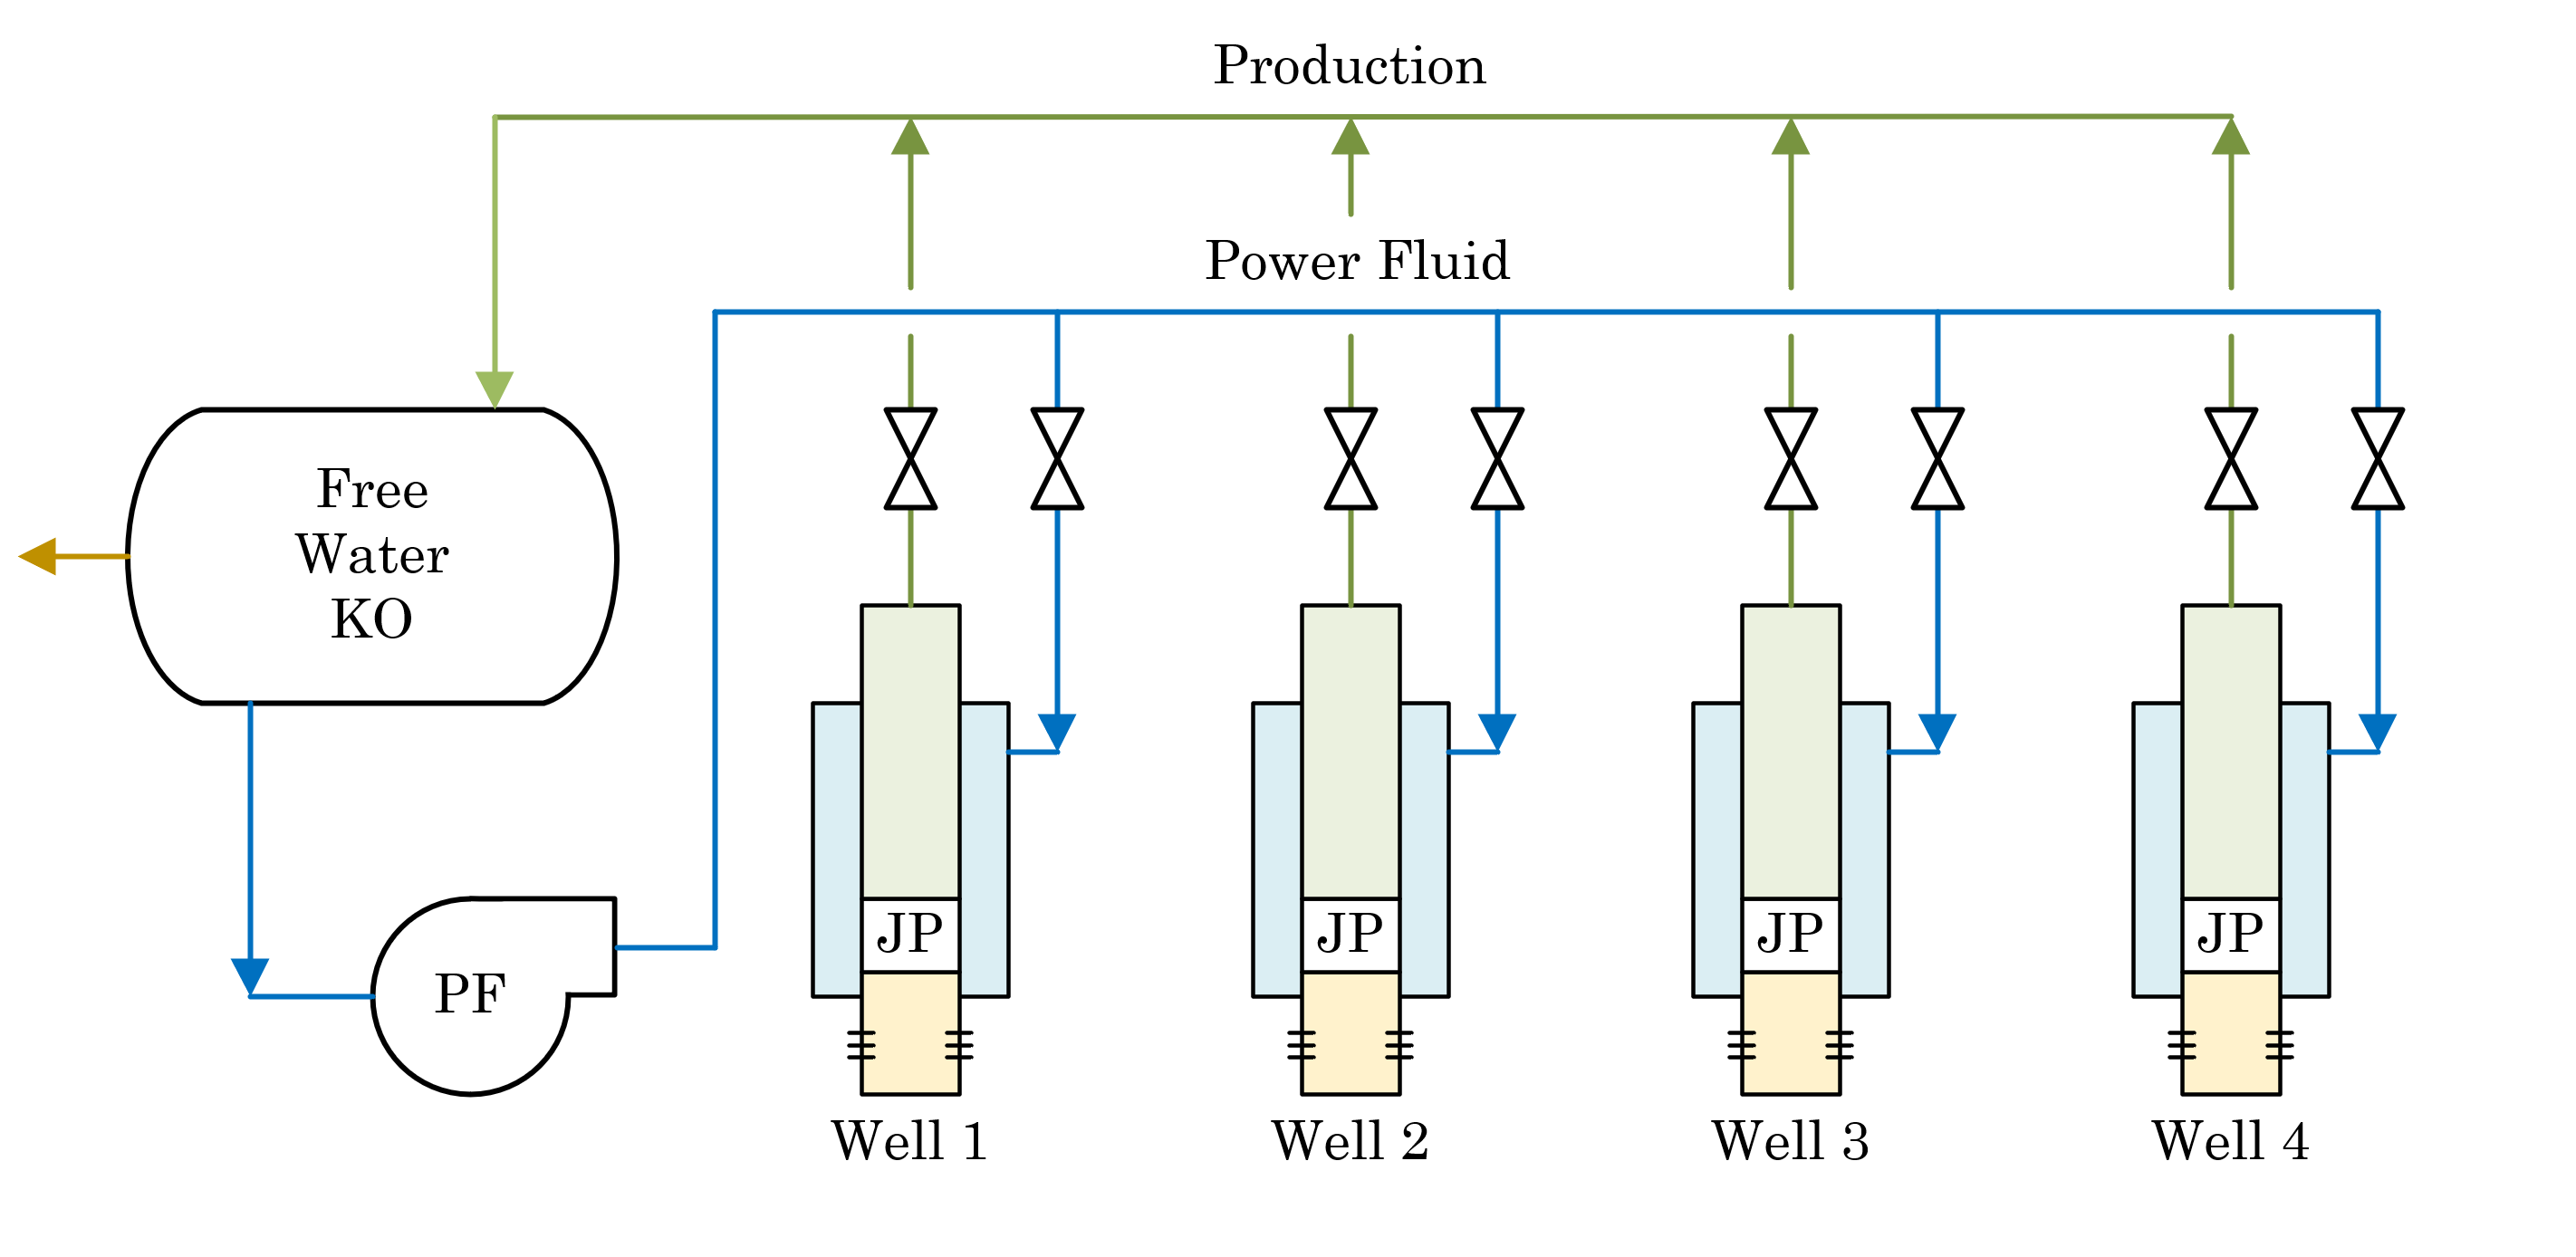
\includegraphics[width=1\linewidth]{figures/network_diagram.PNG}
    \caption{Network Diagram of Four Wells}
    \label{fig:jetpump_network_2}
\end{figure}

\begin{equation}
    q_{oil} = q_{\text{max}} \left( 1 - 0.2 \frac{p_{res}}{p_{su}} - 0.8 \left(\frac{p_{res}}{p_{su}}\right)^{2} \right)
\end{equation}

\begin{equation}
% The vphantom gets the vertical alignment of the underbraces
dE_{te} = \int_{su}^{te} \frac{dP}{\rho} + \frac{v_{te}^{2}}{2} * (1+K_{en}) = 0
\label{entr_intg}
\end{equation}

\begin{equation}
P_{te} = P_{ni} - \frac{\rho_{nz}v_{nz}^2}{2}*(1+K_{nz})
\label{nozz_pte}
\end{equation}

\begin{equation}
P_{te} - P_{tm} = \frac{\rho_{tm}v_{tm}^{2}K_{th}}{2} 
 + \frac{m_{tm}v_{tm}}{A_{th}} - \frac{m_{nz}v_{nz}}{A_{th}} - \frac{m_{te}v_{te}}{A_{th}}
\label{throat}
\end{equation}

\begin{equation}
% The vphantom gets the vertical alignment of the underbraces
dE_{di} = \int_{tm}^{di} \frac{dP}{\rho} + \frac{v_{di}^{2}}{2} - \frac{v_{tm}^{2}}{2} * (1+K_{di}) = 0
\label{diff_intg}
\end{equation}

\begin{equation}
P_{di}^R = P_{wh} + P_{fric} + P_{static}
\label{pdi_req}
\end{equation}

\begin{equation}
R_{di} = P_{di}^A - P_{di}^R
\label{res_disch}
\end{equation}

\begin{equation*}
\begin{align}
    q_{\text{pf}} &= v_{nz} A_{nz} \\
    A_{nz} &= \frac{\pi d_{nz}^{2}}{4} \\
    v_{te} &= \frac{q_{oil}+q_{wat}+q_{gas}}{A_{te}} \\
    A_{te} &= A_{th} - A_{nz} \\
    A_{th} &= \frac{\pi (r_{th}d_{nz})^{2}}{4}
\end{align}
\end{equation*}

\section{Nelder-Mead Application}

Solve the equations shown above to find a solution for a given nozzle and throat ratio. Apply the Nelder Mead to choose different nozzle diameters and throat ratios in an attempt to maximize the produced oil while staying under the allowable power fluid demand.

\begin{equation*}
\begin{aligned}
    \text{maximize } & \sum_{i=1}^{k} q_{\text{oil}}^{i} \\
    \text{subject to } & \sum_{i=1}^{k} q_{\text{pf}}^{i} \leq Q_{\text{pf}}^{\text{pump}} \\
    & q_{\text{pf}}^{i} \geq 0 \\
    \text{Nozzle Diameter: } & 0.1145" \leq \text{d}_{\text{nz}}^{i} \leq 0.3404"  \\
    \text{Throat Ratio: } &  1.44 \leq \text{r}_{\text{th}}^{i} \leq 2.63
\end{aligned}
\end{equation*}

\section{Simple Curve Fit}

Curve fit the discrete finalist of jet pumps. Left with the equation 

\begin{equation*}
    q_{oil} = c_{1} - c_{2} \exp{(-q_{pf} c_{3})}
\end{equation*}

Where $c_{1}$, $c_{2}$ and $c_{3}$ are curve fit coefficients.

\begin{equation*}
\begin{aligned}
    \text{maximize } & \sum_{i=1}^{k} q_{\text{oil}}^{i} \\
    \text{subject to } & \sum_{i=1}^{k} q_{\text{pf}}^{i} \leq Q_{\text{pf}}^{\text{pump}} \\
    & q_{\text{pf}}^{i} \geq 0 \\
\end{aligned}
\end{equation*}

Would follow the method to that outlined in the paper I sent you, most likely using actual derivatives. Add some math at the end to actual choose the discrete jet pumps.

\cite{gas_lift_econ} and \cite{gas_lift_quasi}

\printbibliography

\end{document}